\documentclass{article}
\usepackage[utf8]{inputenc}
\usepackage{graphicx}
\usepackage{hyperref}
\usepackage{nameref}


\hypersetup{
    colorlinks=true,
    linkcolor=black,
    filecolor=magenta,      
    urlcolor=blue,
    citecolor=red,
    pdftitle={Overleaf Example},
    pdfpagemode=FullScreen,
    }
    
    
\title{Neural Networks in the financial market:\\ Backtesting and automation}
\author{Daniel Schussmann \\ HTW-Berlin }
\date{2022}


\begin{document}



\maketitle




\section*{ABSTRACT}

The aim of this project was to figure out whether a A.I. trading bot is a feasible idea or not. To achieve this, financial foreign-exchange-market data was gathered from the web and then pipe-lined into several different neural networks to be trained. Afterwards the trained neural networks were evaluated using a back-testing environment. The goal of the back-test was to conclude if the neural net was able to learn a real world applicable strategy to profitably trade the forex market. All the trained networks were basic, feed forward networks\cite{MLB112} with the main difference being the neuron count. As expected from \cite{overfit} \cite{MLB123} other works on the topic, both over- and under-fitting were a problem. The golden middle showed promise at first, but after evaluating the backtesting results there seemed to be no evidence to believe that the network acted by strategy rather than pure chance.

\section*{KEYWORDS}
artificial-neural-network, trading-bot, back-testing, Artificial-intelligence-trading


\section{INTRODUCTION}
Artificial intelligence is soaring in popularity, with job offers and opportunities in abundance. Although the base principals of artificial intelligence have been introduced by Alan Touring back in 1948\cite{father}, we are however still on the fore front of realising it's full potential. This being said, A.I.'s are used in most tech-industries and are almost impossible to work without. This is shown by the rise of AI manufacturing which is rapidly turning into the industry standard. \\~\\ Trading in centralized markets started sometime in the 13th - 14th century in Antwerp.\cite{finhist} Since their invention they have changed and adapted frequently.\cite{marketevo} Especially the evolution of technical analysis gave reign to a multitude of indicators and strategies, which aim to predict and therefore exploit the movement of the market. A market is a system in which an item is traded. The item can be real commodities like gold, virtual currency like bitcoin or company shares like stocks. This project focuses on the euro-majors. Most currencies of the world are traded in the foreign exchange market(FOREX), in this context, majors are the currencies which have the highest trading volume and are therefore the most influential. They include(name - followed by short): the EMU\footnote{Economic and Monetary Union}-euro(EUR), the United states-dollar(USD), the Japanese-yen(JPY), the British-pound-sterling(GBP), the Australian-dollar(AUD), the Swiss-franc(CHF), the Canadian-dollar(CAD) and the New Zealand-dollar(NZD). I choose this type of financial instrument, firstly because I am familiar with this market, as I have been trading it for a while, secondly, because It's very versatile and actively traded, which means there are millions of trades happening a second, making high frequency trading\footnote{trading in time frames below, or at 1H} stable and viable.\\~\\Neural networks are networks comprised of neurons. The term neuron is a metaphor for real neurons present in human brains. There are however not have many direct similarities besides the name. A neuron can be imagined as a node, which holds a value, usually a number between one and zero. The value itself indicates the power(importance) of the neuron. In a neural network, neurons are arranged in layers which connect to each other. The connections are called weights and they can be arranged in a multitude of ways \cite{structure}. For this project the standard form of neural networks was used, which means every neuron is connect to every neuron in the next layer sequentially.
%\autoref{fig:neuralnet}
\begin{figure}[!h]
\centering
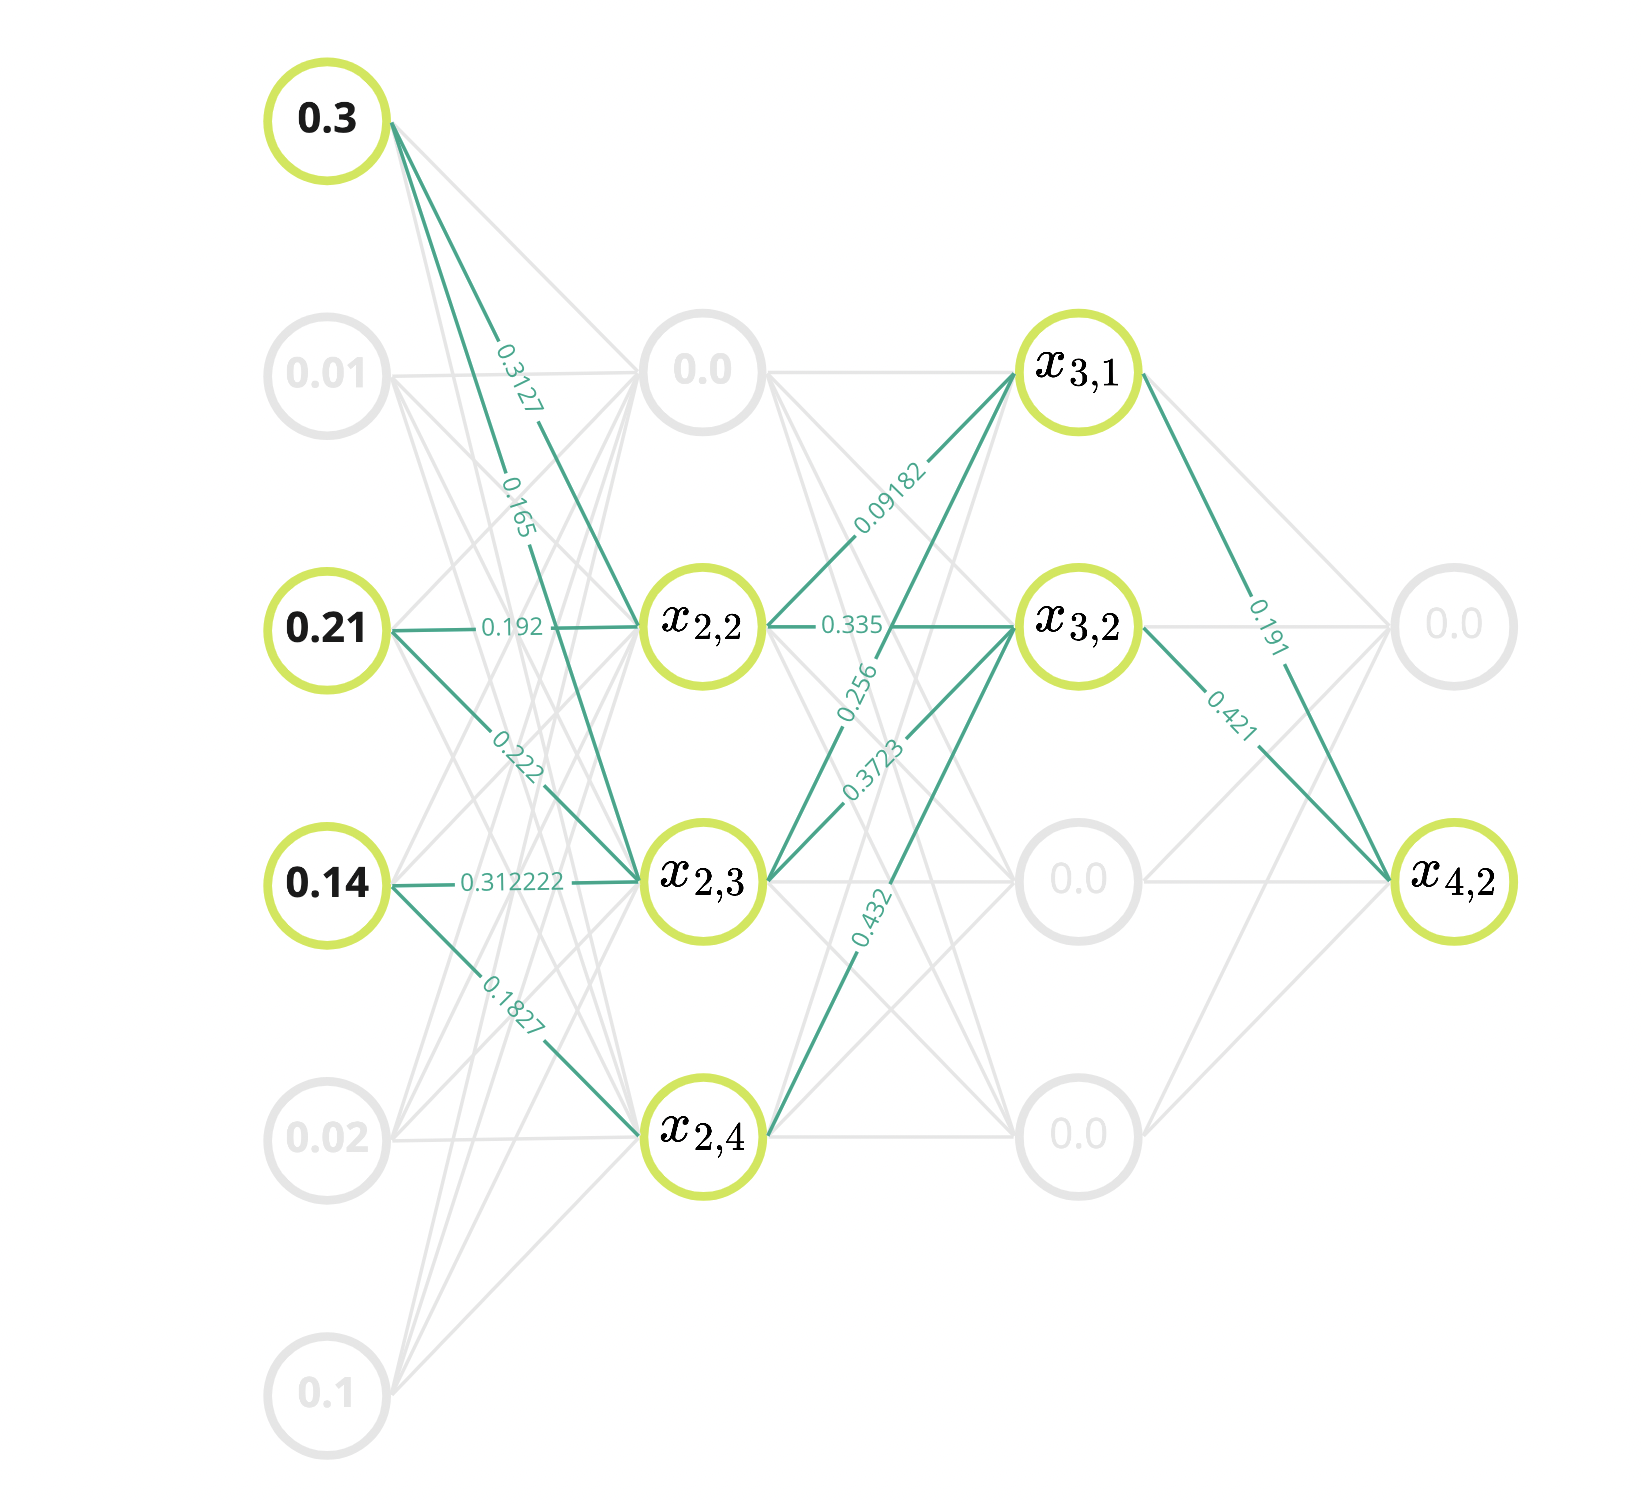
\includegraphics[scale=0.24]{netimage.png}
\caption{\label{fig:neuralnet}An example structure of a neural network}
\end{figure}
\pagebreak
Each neuron also has an individual bias assigned, to further randomize the power of each neuron and give the best chance of learning. The value of a neuron is the combination of all the values of the neurons feeding into it multiplied my be respective weight. More about the basics of neural networks \cite{intro}. The essential workflow of a feed forward neural network is comprised of feeding data into the input layer and then letting the neural network produce an output, which is in the manner of its training sets. For this project the input data is forex data, and the sought after output is a prediction of long or short. More closely an output which should look like this: [0.123,0.831], where the first value represents the certainty of the network to short and the second value the certainty to long.\\~\\
In the process of evaluation, a backtesting framework will be used to test the performance of the neural networks trading predictions. Backtesting is a common method for test running a system, if feasible data of the past is available. It therefore is commonly used for trading, because every second of market change is recorded and readily accessible. A backtest in the case of this project can be seen as simulating a broker, whilst simultaneously controlling the market movement. A broker in the sense of instance which is able to execute and close trades, where the profit or loss is automatically calculated. And controlling market movements in the sense of providing the price movement of a symbol artificially in a much faster speed then reality, more on this in the methods section. For a successful backtest ground rules need to be set: A starting budget of 10000€ is set, as well as a set order size of 200 and a leverage\footnote{ leveraging can be compared to lending, so for every euro you invest the broker lends you 50, which allows a trader to make more versatile trades} of 50, fees and taxes are ignored for the sake of simplicity. When an order is made the direction is required for execution, which means a long or short definition is needed. The showcased simulation ran for 3000 ticks to make the output more visually appealing. Since every amount above 3500 is to much for the server to still produce a pleasing viewing experience. 

 



\section{METHODS}
Firstly financial forex data had to be gathered. The whole data was consistently downloaded from the website https://www.dukascopy.com. All data sets are in the hourly format, meaning price changes are indicated by the hour. The data structure is candle like, meaning open, close, high and low are the data points. As exchange pairs, EUR/USD, EUR/CHF, EUR/GBP, EUR/AUD and EUR/JPY have been used. The time frame of the data was 2 years. To compile this information shortly: hourly forex candle data for various euro pairs in a time frame of two years, has been gathered from dukascopy. The file type was .csv meaning comma separated list, because it can easily be checked in excel. Furthermore, with csv, rogue values can be quickly identified and swiftly deleted. It is important to note that flat values have been filtered from the data. Flat values are times when the market is down, ergo when there is no movement over several steps. This includes weekends(the foreign exchange market closes on weekends), general closing times, national holidays and more rare events. The filtration of flats is important because the later trained neural network will struggle with a not moving market, because it does not understand that the market is frozen. Since there is no point in trading a closed market, because no profit can be made, implementing a way for the neural network to identify when the market is down was redundant, filtering flats was the best solution. Now the filtered data had to be prepared for the neural network, because feeding it directly does not work. This stems from the general functionality of a neural network, where it is impossible to train a neural network on highly fluctuating data, because neuron importance's is tied to the magnitude of the value. Higher values are viewed as more important by the network, while lower values are categorised as less influential. For data preparation the \href{https://colab.research.google.com/drive/1KucTlScag3R0D2piUODHtQ1eAmDSQ2Rv#scrollTo=9AWlOIJSpKvO}{mean\_movement()} class has been used, it requires two parameters: "inputfile","columns" which refer to the file from which the data points are supposed to be pulled from, as well as the columns to use. Columns are as described above, open, close, high and low. After these two parameters have been passed the data is converted into a pandas data frame, for ease of manipulation. Following, the data frame is sectioned into 10 sets of data points, e.g. if there were 2000 unsorted data points, now there are 10 * 200 sets of data points. In the next step, the individual batches are normalized using basic matrix normalization, with the \href{https://colab.research.google.com/drive/1KucTlScag3R0D2piUODHtQ1eAmDSQ2Rv#scrollTo=gcF9CM1Tuaib}{normalize()} function. The normalize function normalizes the 1x10 matrix in three steps, firstly it squares every value and stores the resulting vector in the A variable, secondly it sums all the values in A up, takes the root and stores the result in the v vector, lastly every original value is divided by v. The resulting vectors override the original data frame which is now filled with normalized batches. In the next step the batches are split into even and odd, where even sets are stored in x\_norm and odd sets are stored in y\_norm. The final line of the function then returns both x\_norm, y\_norm, the normalized batches and the raw data. The big picture is now that the first value of x\_norm directly co-responds to the first value of y\_norm. For clarification, x\_norm[0] is filled with the first 10, normalized, data points from the original data source and y\_norm[0] is filled with the second 10, normalized, data points. Now x\_norm represents the training data, meaning the data which is shown to the neural network. y\_norm has to be modified and will hold the example results, so the prediction examples the neural network should stride to replicate. This modification was also achieved by the mean\_movement() function which takes the passed values, calculates the mean and then simply checks if the mean price went up or if it went down. If price is above the first value the function assigns the value of 1 to the batch, which means a buy order would be viable, respectively the function assigns a 0 if price went down and a sell order would be the better option. With the latter step, data preparation is finished and the data frames x\_norm and y\_norm can be fed into the neural network. The neural network itself is created using the \href{https://colab.research.google.com/drive/1KucTlScag3R0D2piUODHtQ1eAmDSQ2Rv#scrollTo=jxYWLBJjbARf}{NeuralNetwork()} class, which works as follows. After being initialized the first step is to create all the required layers using the add\_layer() method. Several layer types can be used but a certain order is required, because the network type is sequential, which means layers are arranged in sequence and one directly feeds into the next one. The first layer needs to be set as type "Input" and the last layer has to be of type "Output", for the neural network to recognize the start and end of the structure. With the two already explained layer types being simple and straight forward, lets begin explaining the more versatile layer type of "Dense", or "hidden" as I reference it in the code. Dense layers have neuron counts just like input and output layers, but they have a few additional parameters: the activation function and initializers. Initializers are essentially randomizers, which randomize the values of weights and biases on a predefined basis. This practice yields better results \cite{init}. The activation function can be chosen freely but some make less sense then others. Popular activation functions include tanh, sigmoid, relu, elu etc.\cite{activation}). During the evolution of this project many different functions were tested but the in the end the relu function was chosen, because it showed the highest accuracy, out of the ones that were tried.
After all the layers have been successfully added, the compile() method can be called OPTIONALLY. This not required method returns insight on the number of trainable parameters, the layer sequence and the overall setup. This was used extensively whilst testing, but has no real use in the final version because terminal outputs can not be viewed by the Backtesting framework.\begin{figure}[!h]
    \centering
    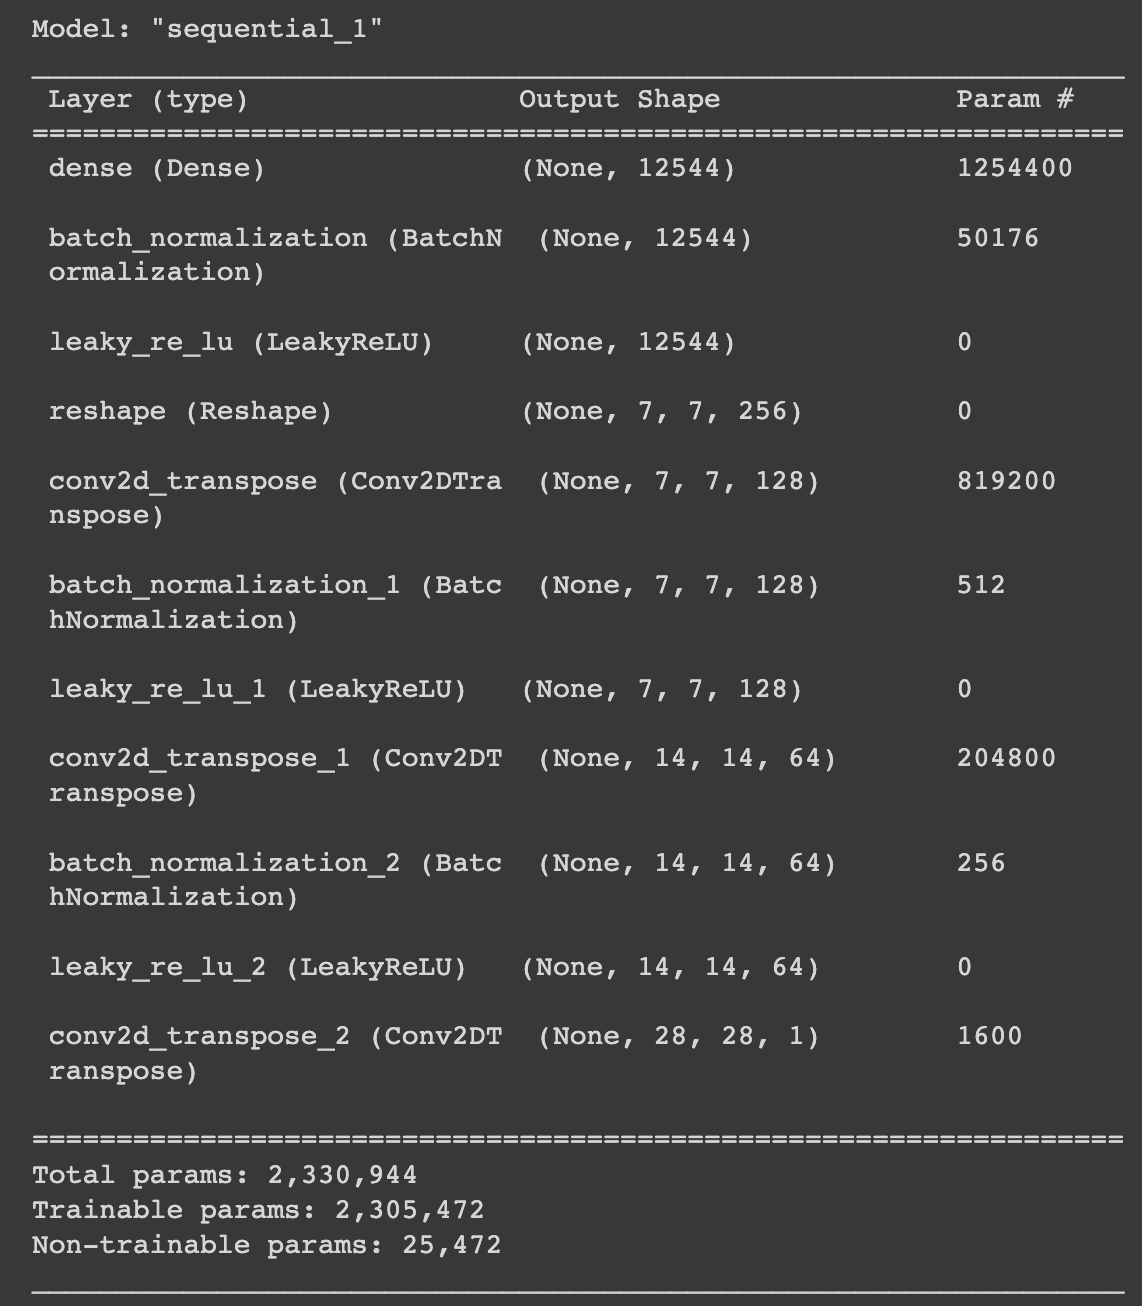
\includegraphics[scale=0.3]{NETWORKSTRUCUTRE.png}
    \label{fig:struct}
    \caption{Example output of the complie() method}
\end{figure}
\newline
The next method that should be called is the prep\_data() method. This method simply splits the passed data into two and stores one half in the training variable and the other half in the validation variable. This is a necessary step when using the tensorflow framework, because in the following fitting process the neural network will be trained on the training data, whilst being validated constantly on the validation data. This means the network is never trained on the validation data and never validated on the training data. Therefore an evaluation of the accuracy of the neural net can be taken while it is being trained without risking the neural network learning from validation data. This results in graphs which show the learning processes and how the accuracy and the loss \cite{loss} changed over time.
\begin{figure}[!h]
    \centering
    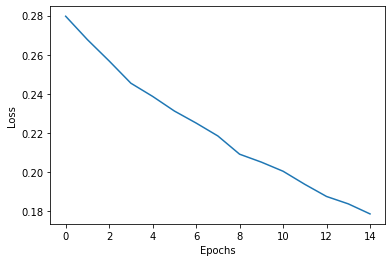
\includegraphics[scale=0.6]{loss_im.png}
    \label{fig:loss}
    \caption{Example loss progression over training period of 15 epochs}
\end{figure}
\newline
As already briefly mentioned above the next step is fitting. This was achieved using the Fit() method. Fitting is the technical neural network  term for training. "The code for the fitting process is short, but regardless of its length this is where the majority of all the action happens." The tensorflow fit() function trains the neural network by showing it an input, in our case the set of market data points, followed by the associated result. As mentioned before this is x\_norm and y\_norm. The network then adapts its weights and biases with every example, to gravitate towards being able to mimic the output. Every few changes the network validates the networks progress with the validation data and then alters learning rate on the running accuracy. Depending on the network complexity and the amount of epochs, which means repetitions of learning, this can take a few seconds to minutes. When using the right configuration the result is a fitted and functional neural network that returns a plausible output to an OKAY input. The last used method of this class is the save method. This method saves the exact trained neural network with all its parameters, so it can be used without having to rebuild everytime a prediction needs to made. By setting tensorflow.keras.load(neural network) equal to a variable, the variable can then be called with an input and it will produce a prediction. 
\newline
The final part of the project was the back testing framework. Backtesting was done by the \href{https://colab.research.google.com/drive/1KucTlScag3R0D2piUODHtQ1eAmDSQ2Rv#scrollTo=MXbGIyR4KJiJ}{BACKTEST\_v3()} class. Unlike the Neural Network builder class, the BACKTEST\_v3() class is fairly complex and it would be overblown to explained every aspect of it. A simplified explanation of the BACKTEST\_v3() referenced as BT follows. The BT class allows four methods to be called after initiation: tick(), MakeOrder(), SellOrder() and Draw(). tick() is the first described method and its main function is to emulate the passing of time. A normal financial market moves on its own, every second, hour, day the market updates. Now for a simulation of data which passed over two years, waiting for an hour before loading new data would not be a good approach because simulation time would take two years. That's why new data is loaded by the tick() function every time it is called. With this setup a week worth of data points can be scanned through in seconds using for loops. The technical process can be imagined as: two years of data-set is passed to the class, the self.index variable indicates -the moment of time / -the position in the data-set. At initiation the self.index is at zero so at the first data point, now every time the tick() method is called the self.index variable increase by one. This means the reference of data[self.index] moves to the next index in the data(the next candle). Now that price movement can be simulated, trades need to be executable. For this the MakeOrder() method is used. It firstly checks for errors in the call, then it assigns the buy price, the execution point(to the exe\_id), the hash for referencing(to the hax variable) and finally the order is created by adding a new dictionary key to the open\_orders dict. The parameters that are passed, symbol, o\_type and note, tell the BT class what type of order should be placed, while having the option to leave a note for later troubleshooting. It is very important to note that the MakeOrder() method also returns the individual hash, which is a time based hexadecimal hash, at the very end of the function, so it can be referenced when the order is bound to be sold. The open\_orders dict key for the created order is the hash as well, which makes it very easy to be referenced, by using the code name.open\_orders[hash]. The SellOrder(), as mentioned previously, is called when an order needs to be sold. Which specific order is determined by the hash that was assigned to the order when it was executed. Internally the SellOrder() method calculates the profit or loss of the order by taking the buy prices, which is stored in the open\_order dict, then depending on the order type subtracting buy price from current price, or current price from buy price. After profit or loss are determined the whole order specifications are stored in various sections inside the self.analytics dictionary. The self.analytics dictionary holds all the orders which have been successfully sold, separated by symbol, as well as portfolio changes, which basically means changes in the available cash sum. The final step of the SellOrder() method is to delete the now closed order from the open\_orders dict. All the later methods inside the BT class are used for visualization. \href{https://do-nothing-option.herokuapp.com/}{Backtesting results hosted on a heroku server}. The backtesting overview is comprised of:
\pagebreak
\begin{figure}[!h]
\centering
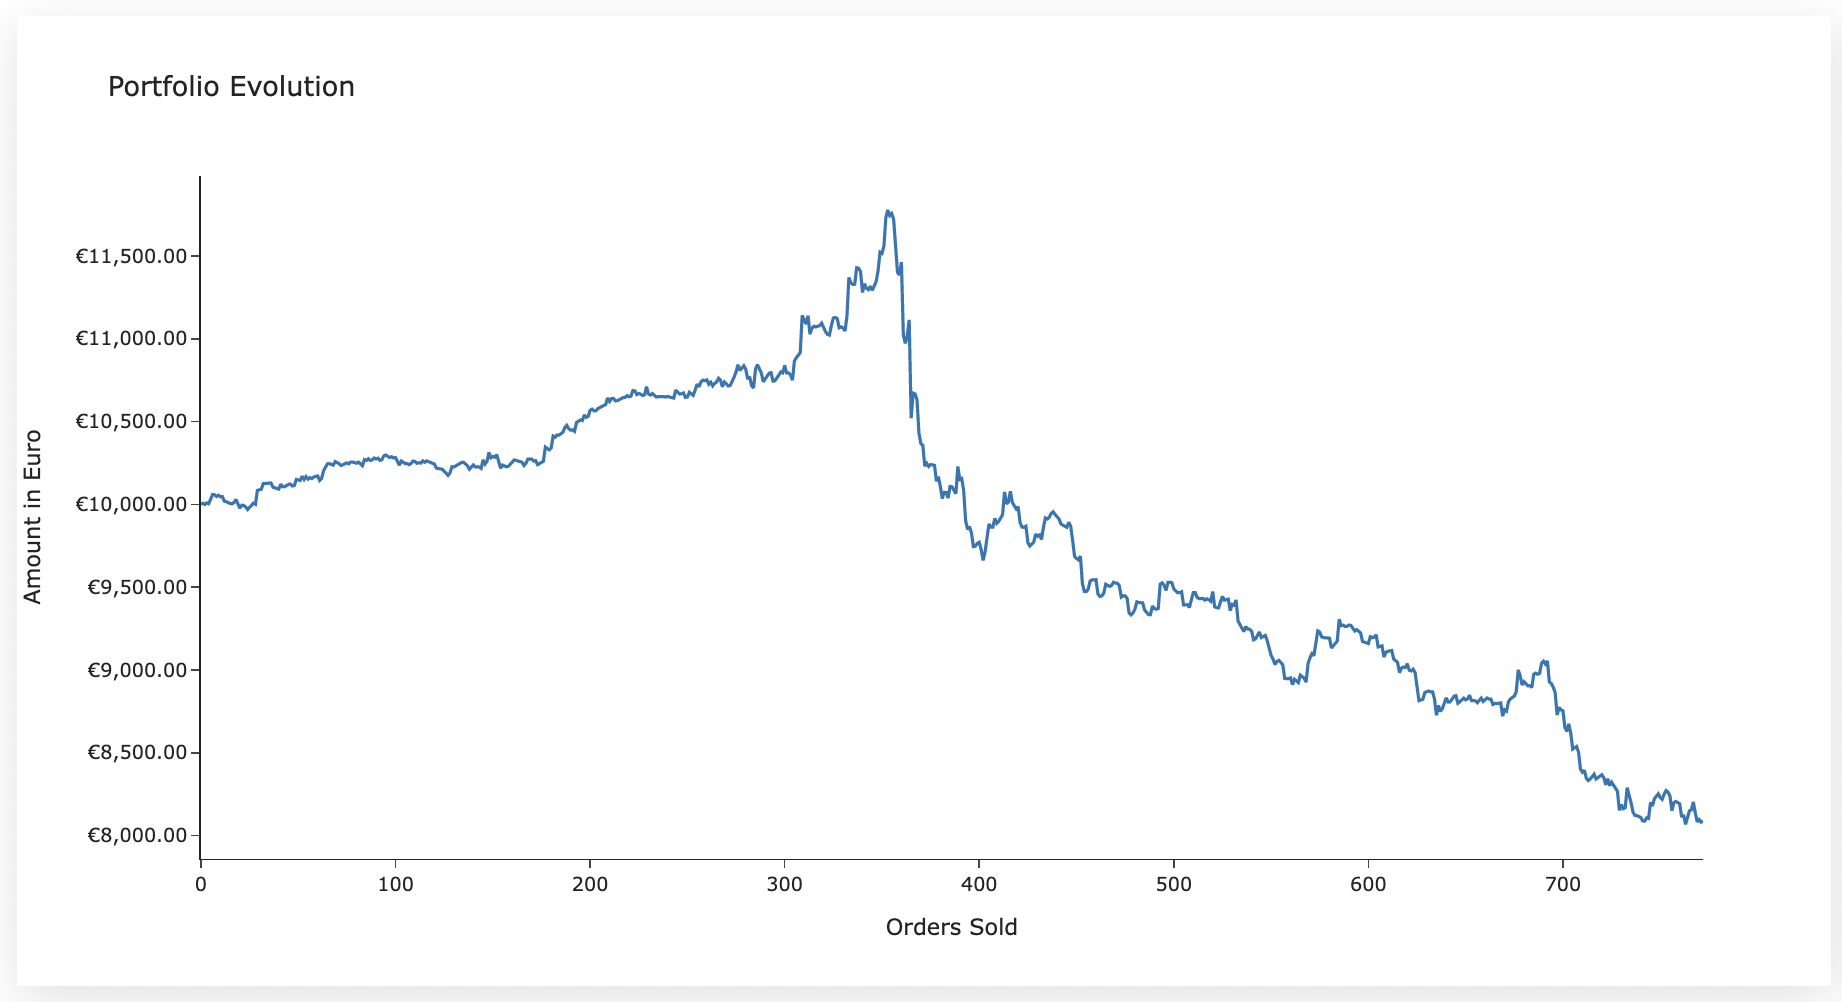
\includegraphics[scale=0.3]{port_evo.png}
\label{fig:portfolio evolution}
\caption{shows the graph of the evolution of the portfolio(balance). Every time a trade is executed a new point is added, it can be hovered to show detailed info about every change. The last entry is the final status of the Backtest. It is produced by the direct pipeline from  self.analytics['portfolio\_mvmt'][symbol]}
\end{figure}

\begin{figure}[!h]
\centering
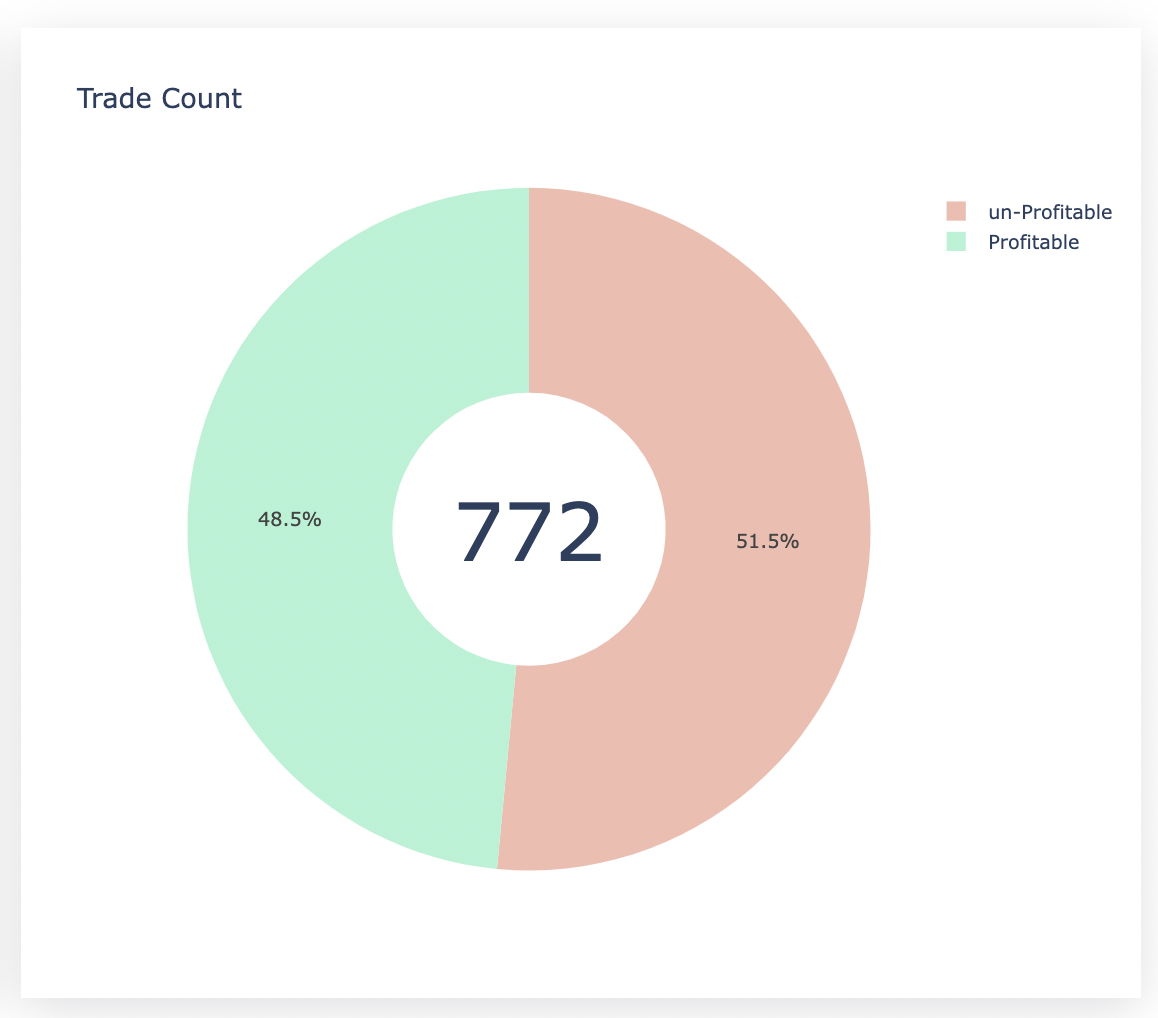
\includegraphics[scale=0.3]{trd_cnt.png}
\label{fig:trade count}
\caption{is the trade count donut chart. It changes if the symbol is switched with the drop down menu. It's center is the total number of trades made, while the outer slices indicated profitable and unprofitable trades. It can be hovered to show the exact number of trades in each category.}
\end{figure}



\begin{figure}[!h]
\centering
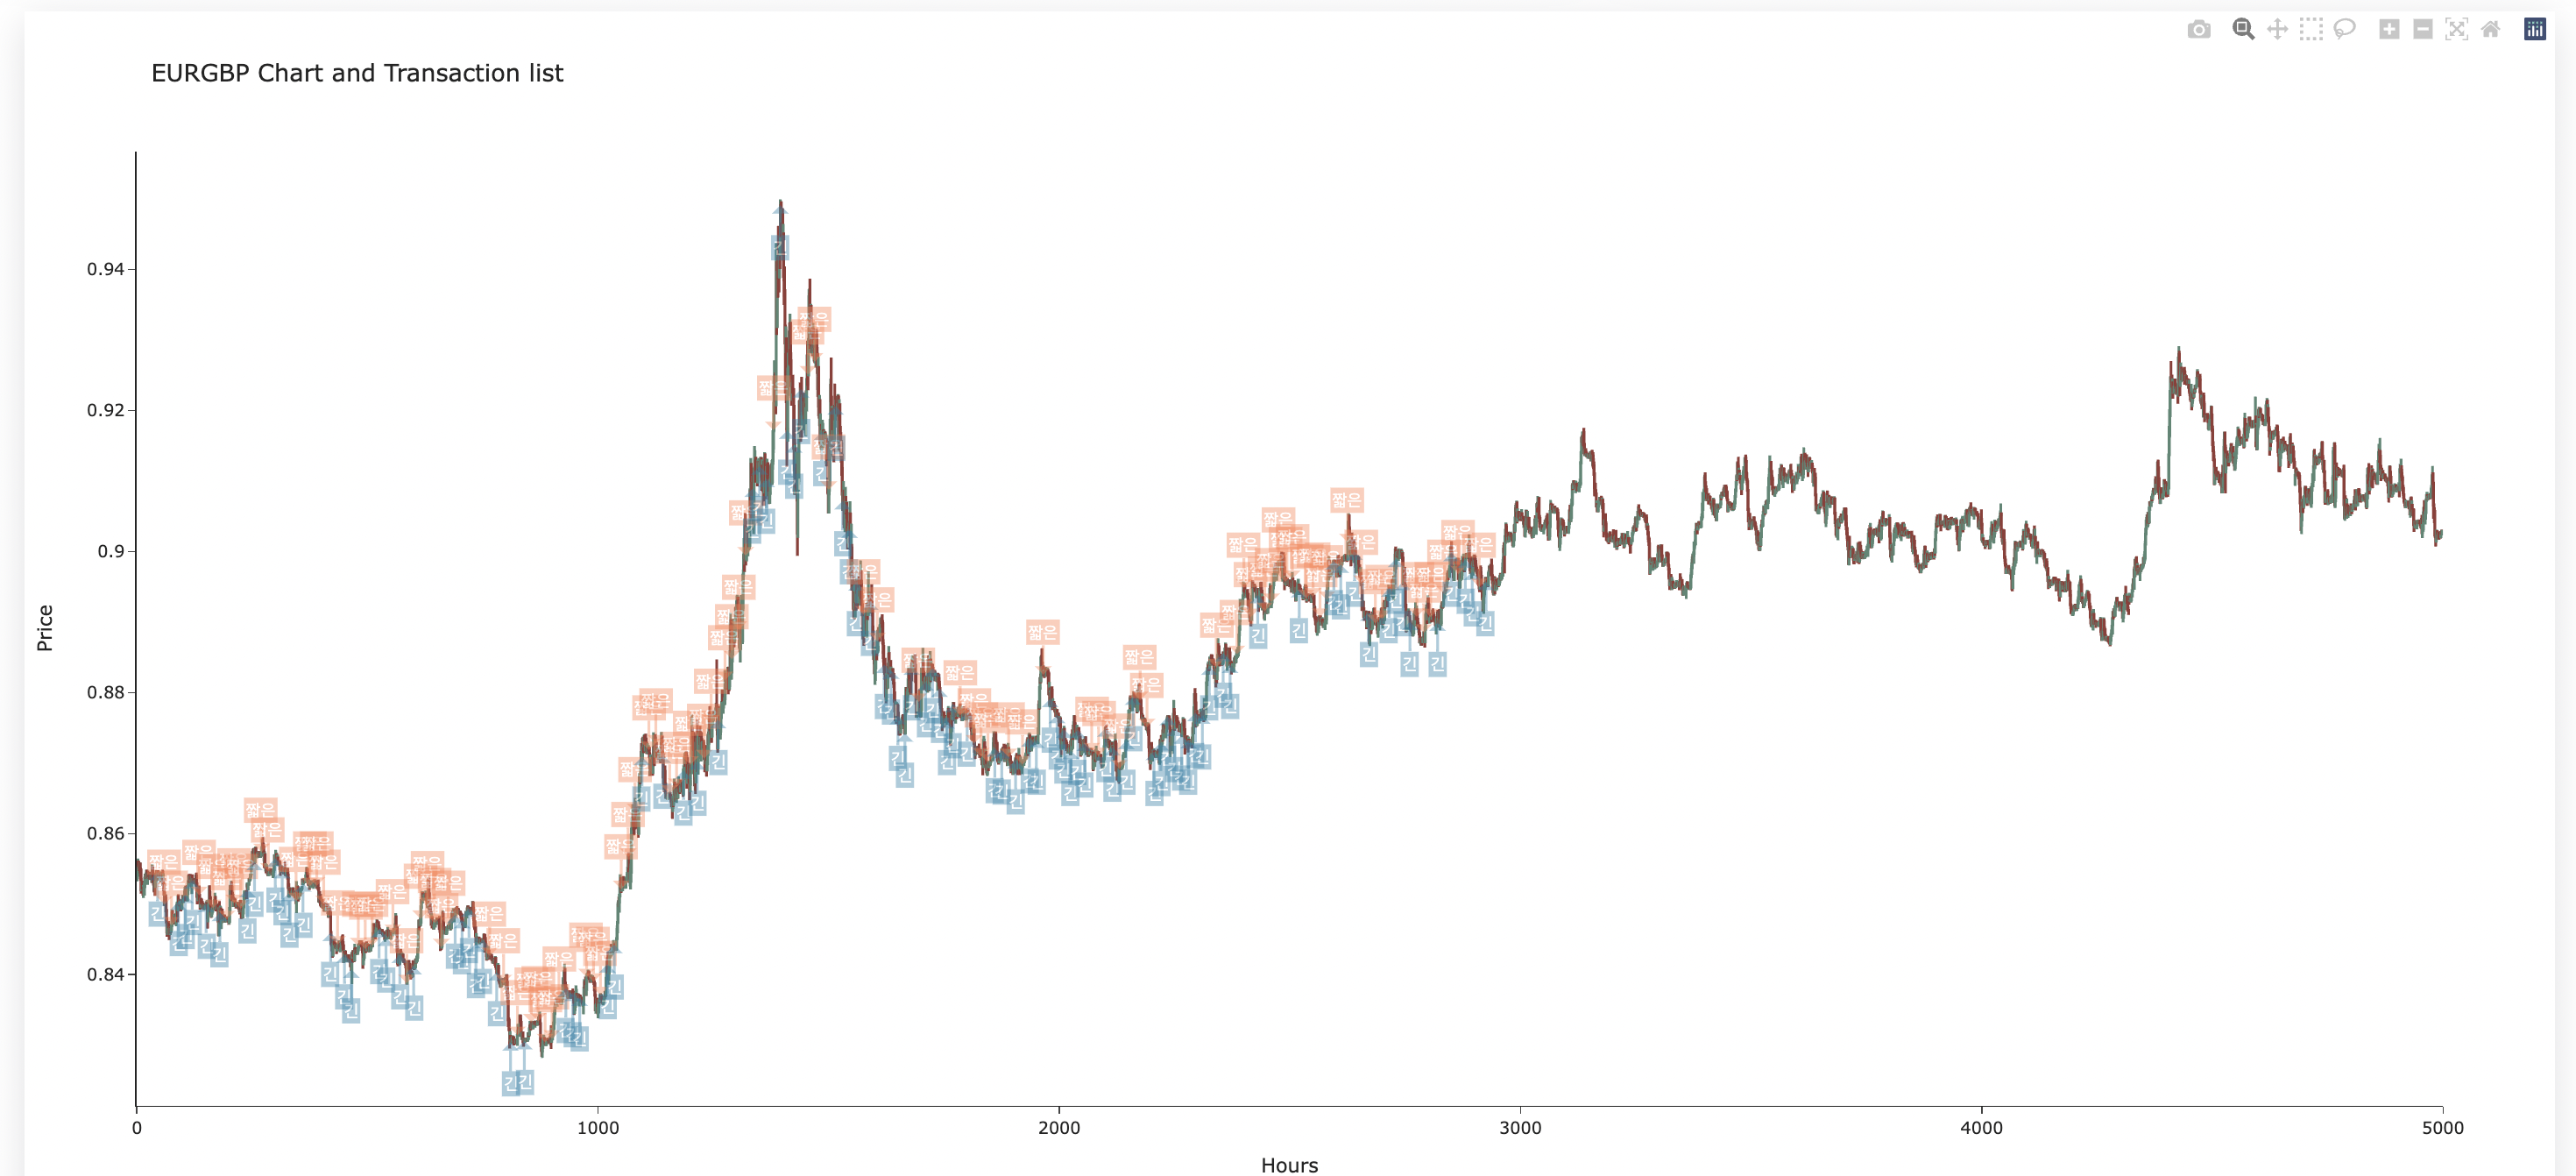
\includegraphics[scale=0.2]{prc_mvt.png}
\label{fig:price movement}
\caption{Shows the candle chart of the selected symbol/s. Long/shorts are indicated by the flags above/below the candles. The candle chart is directly drawn from the used data using builtin plotly functions. The long/short indicators are taken from the self.analytics[symbol] dictionary, by transposing and then indexing the contents.( \href{ https://colab.research.google.com/drive/1KucTlScag3R0D2piUODHtQ1eAmDSQ2Rv#scrollTo=MXbGIyR4KJiJ }{ can be seen on line 219 } ) 
}
\end{figure}



\begin{figure}[!h]
\centering
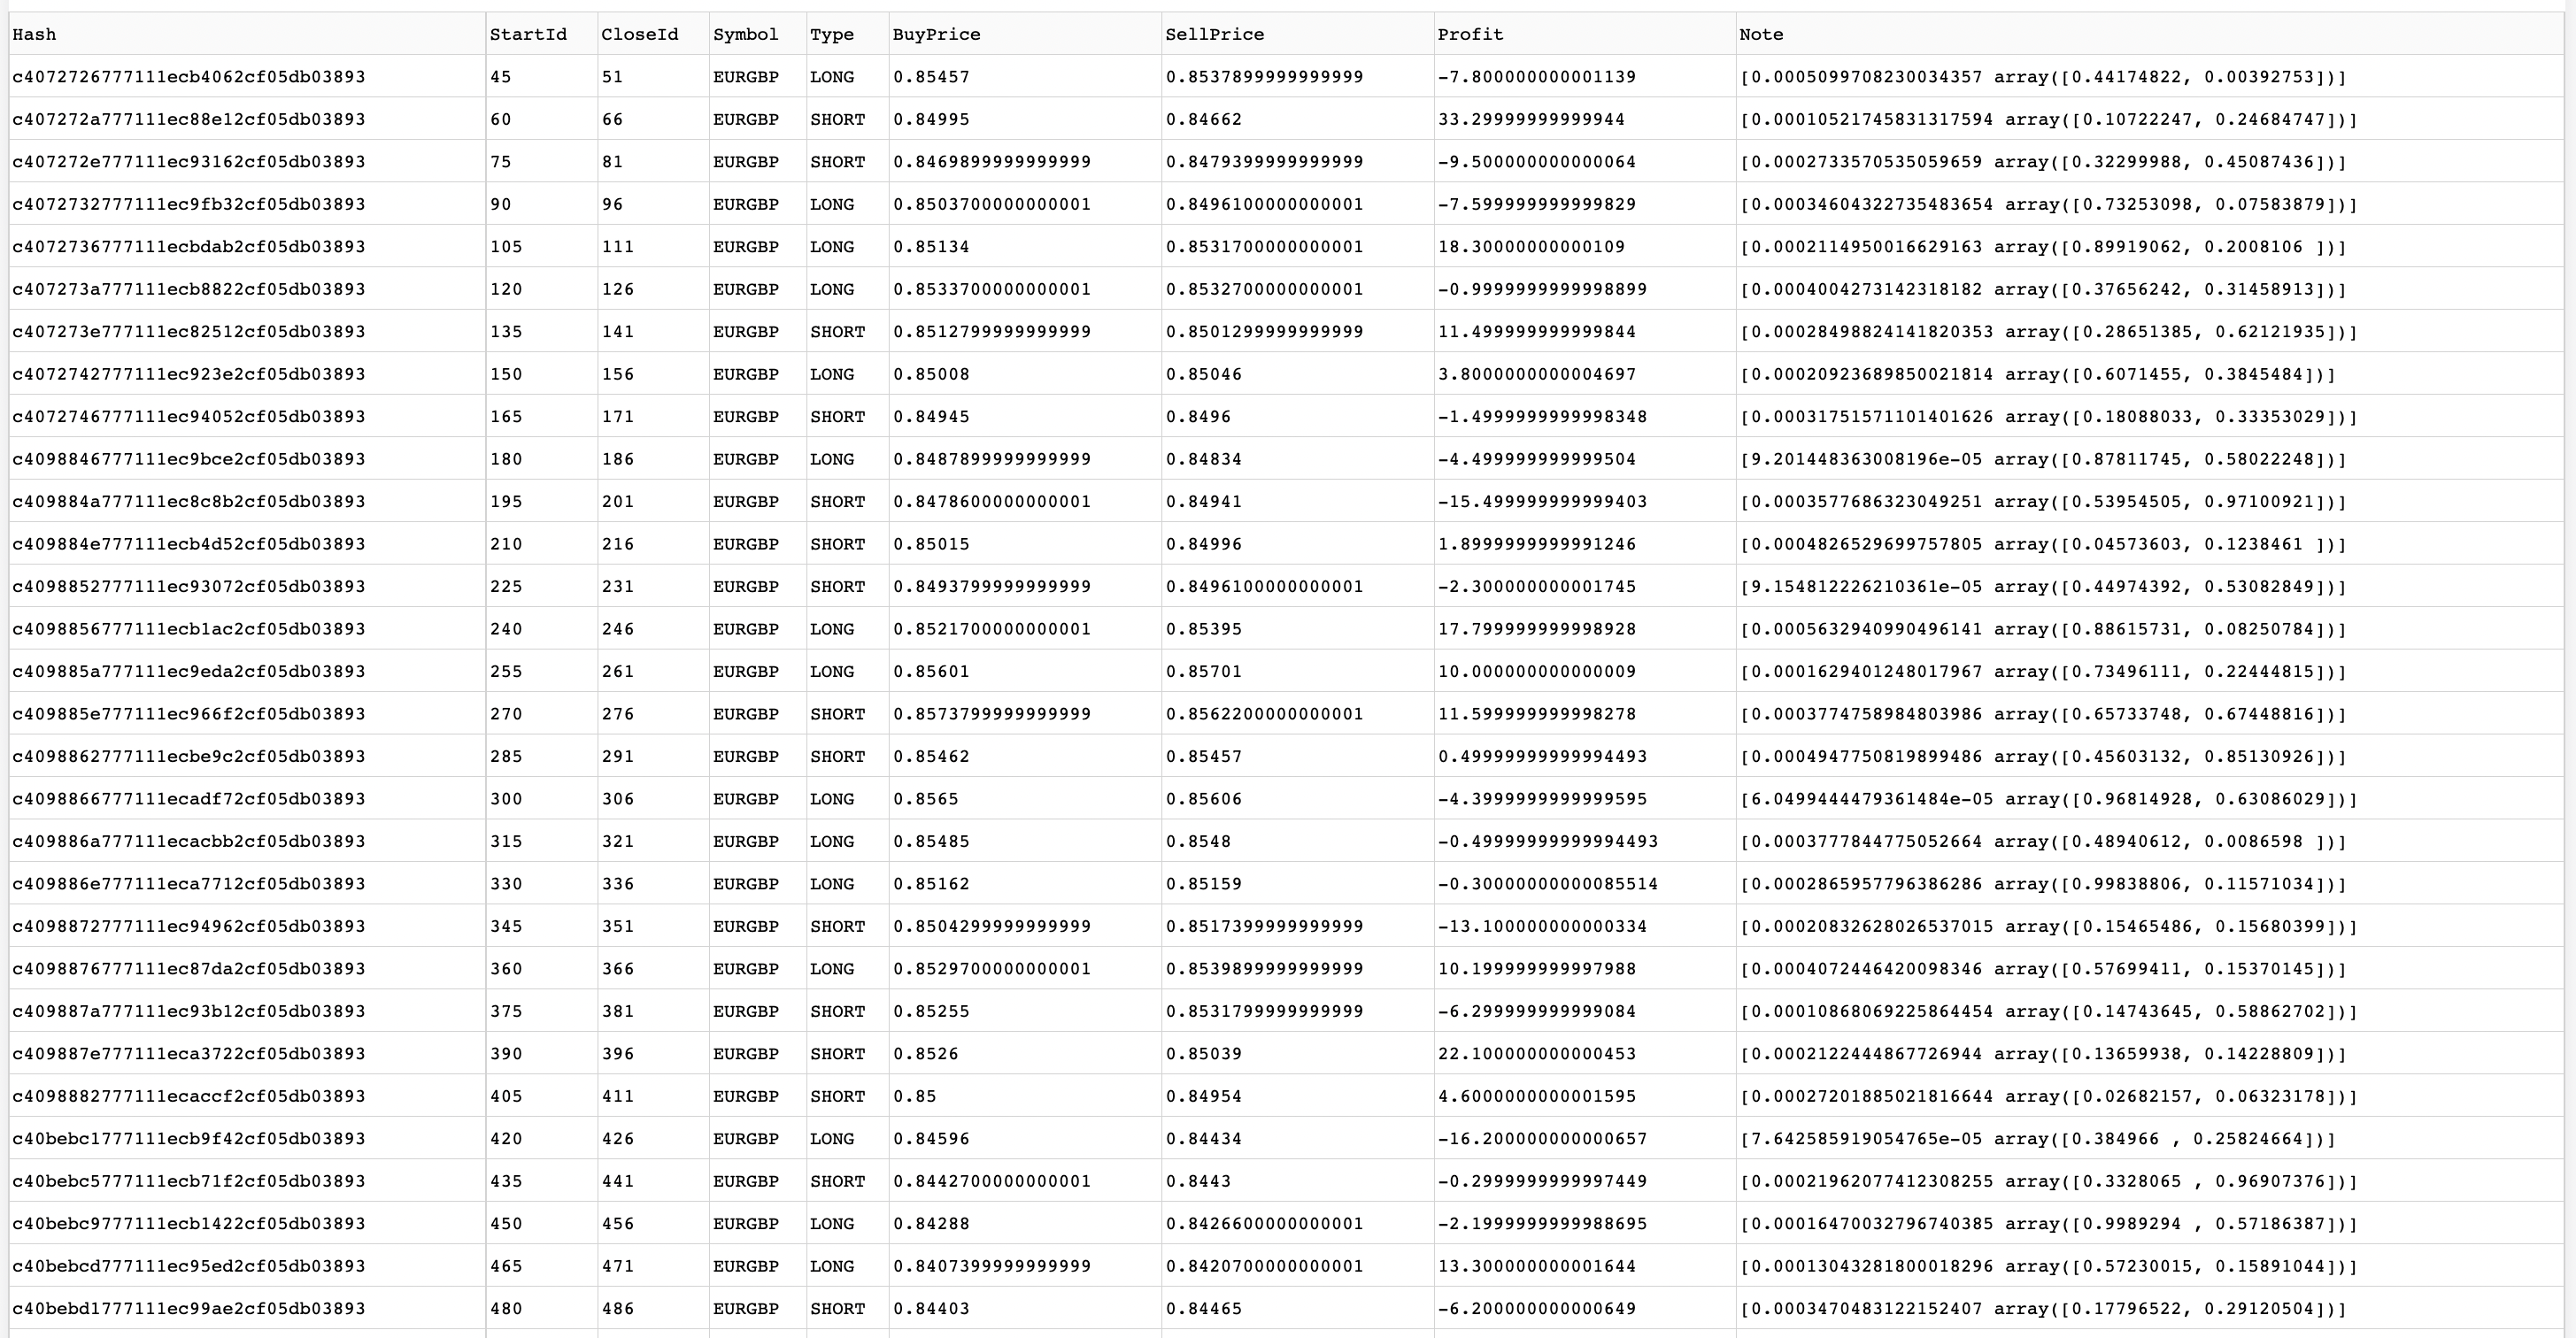
\includegraphics[scale=0.2]{trade_list.png}
\label{fig:trade list}
\caption{is the trade list. It shows all the trades made, with the columns being: Hash, buy/sell id, buy/sell price, the symbol, the order type, the effective profit, and the note. Most importantly for this project is the note which shows standard deviation along with the prediction of the network. The list created by directly converting the self.analytics[symbol] to a table.}
\end{figure} The Backtesting\_v3 class is used in the following snippet \href{https://colab.research.google.com/drive/1KucTlScag3R0D2piUODHtQ1eAmDSQ2Rv#scrollTo=SftgZAoK6tTp}{usage example}
\\~\\

\section{RESULTS}
As supported by the visual of the backtesting framework, the result of the project is a neural network which trades in a set frequency. The showcased neural network was able to produce an output in the admired specifications. This means the output looks like it is supposed to look like, this could be compared to a child writing a random number as the answer to a mathematical question. However the neural network does not produce the results in a meaningful way, it just "knows" that it is supposed to produce outputs in certain format, but not that the output should have a more coherent structure regarding the input. Therefore the overall performance of the neural network was sub optimal, as it was not able to learn / identify patterns and therefore failed to create a valid trading strategy. The final state of the neural network trading strategy performance is comparable to a completely random, non structural algorithmic trading bot, which generates a random number and then uses this number as a prediction. There is no benefit, besides educational learning, in using this neural network for trading. There are many algorithmic trading strategies \cite{betterbot} which produce a much more profitable output and are a lot easier to understand and to create.

\section{DISCUSSION}
The first important topic is the different networks tried. As mentioned before they were feed forward sequential artificial neural networks. All different networks had an input and output layer. Networks which had more or less then two hidden layers had issues with over- or under- fitting. Further any other activation functions lead to the network not producing a feasible output, which means it either was always the same value regardless of the input data, or negative values, or zero. So the final successful network had 40 input neurons in the input layer, two hidden layers comprised of 32 neurons each and an output layer of 2 neurons. This is a very standard composition and its not surprising the other arrangements failed. Focusing on the performance of the neural network that produced promising outputs, it was still apparent that the outputs were not producing a profitable trading strategy. The best explanation for this is the complexity of the data. Neural networks learn well on very tight differences, for example images of cats always look somewhat similar, they have the same features. A financial market is way to chaotic for a simple neural network to find any form of pattern. On some training batches there were close to no similarities in any of the data, therefore learning and evidently finding patterns was impossible. To combat this issue a predefined set of patterns could be identified manually, and then training on these specific batches would yield greater results. However, neural networks need thousands of examples to be able to adjust their parameters in a meaningful way, which means a lot of work for a human in finding and compiling patters. \\~\\ The data gathering worked easily and the quality of the data was good. However it took quite a while to gather. It is recommended to use an API like the FXCM api, which provides all the historical data directly, if a real life usage is in mind. The reason an API wasn't used, is the expensive pricing plans of most services. Despite the data gathering being tedious the pipeline works.\\~\\ The backtesting framework is very basic in its functionality, but regardless of the available options, with a fitting code, it is fully possible to reproduce the process of a broker. The tweaking and adjusting of features took a long time and it would be and probably will be a great tool to evaluate future trading bots. Depending on the setup a multitude of different strategies can be tested with the framework. This being said, stop loss or take profit have to be checked manually, where a normal broker would do this automatically if a limit order is executed. Using different types of orders was experimented with, but the complexity of the implementation out-reigned the benefits for this project, future implementation is planed however. A different algorithm was tested with the backtesting framework, which was a simple harmonic strategy for which the framework served as a great testing ground. However, some features were left out due to time constraints, like a live playback of all the trades. \\~\\ Finally a discussion about effectiveness of the whole system in regards to computation, is in order. The classes and functions were programmed from scratch, which means they are not optimized or specialized. Adding to this is the already slow compiling time of python. This results in a extensive computation time for the complete code. After the neural network was saved and loaded the time is reduced significantly, but large time frames still take a while to be simulated, especially if a somewhat complex trading strategy is in play. This sadly limits the sought after high frequency capabilities to time frames above 30min and only a few markets at once. The performance can however be scaled by using high powered servers, or professionally optimizing the code. Also improvable is the backtesting overview, which uses the dash library. It is meant for small to medium sized projects and can not handle the amount of data points wanted. Programming a display library from scratch could solve this issue.   


\section{CONCLUSION}
The programming of a backtesting framework, a neural network class and the data pipeline were a personal success and will play a role in future projects. However the project itself does not achieve the desired breakthrough in AI usage on the Financial market. The neural networks that were used made decisions randomly, without a feasible pattern or path, which is also reflected in the backtesting results: Almost all b-tests gave a spread of 50/50 in regards to profitable and unprofitable trades. The few that had a favored trading outcome, could be traced back to pure luck. After looking through the trades manually it was apparent that the neural networks themselves acted the same way all the others did, but the market was just perfectly aligned to make it seem like there was a Strategy in place. The overall conclusion for this project, is that basic neural networks, as of now, are not able to learn how to trade the Forex-market autonomously, from raw data alone. The time was not wasted though, a lot was learnt and the ambition to find a functioning process still remains. Furthermore, there are new models and system being released frequently, which provide promise for this technology to prosper in the future \cite{betterbot}. 


\section{ACKNOWLEDGMENTS}
This project was part of the Seminar course at the "Hochschule für Wirtschaft und Technik - Berlin", taken in the winter semester 2021/2022, as part of the Business mathematics bachelors program.
\section{REFERENCES}
 
\bibliography{term.bib}
\bibliographystyle{ieeetr}


\end{document}



